%%%%%%%%%%%%%%%%%%%%%%%%%%%%%%%%%%%%%%%%%%%%%%%%%%%%%%%%%%%
%%%%%%%%%%%%%%%%%%%%%%%%%%%%%%%%%%%%%%%%%%%%%%%%%%%%%%%%%%%
\subsection{Material Scientific}
\subsubsection{Solution}
As already indicated in the experimental section the recipe adopted from \cite{Anwar2017} didn't produce any \td{good} results. 
The solution was milky/cloudy and didn't produce homogeneous films. 
Altering the composition, pH, surfactant etc. didn't improve the resulting \gls{zro} layers. 
%- first recipe tried to improve to achieve more restisting layer. by pH value, surface tension and solution ratios (only 10\% change because it was assumed, that the recipe is good and should be improved, but the recipe should be altered thoroughly. two layers were also tried but didn't even pass the visual examination/test/inspection. A curst was produced. 

The sol-gel recipe optimized by \cite{Hu2016} for \ch{Al2O3} worked splendidly for our use even after (not so) minor changes.
%An substantial improvement could be achieved by
The stability of the solution could be increased a lot by replacing the stabilizing agent (\gls{acoh}) with \gls{ipo}.
The stability was inspected visually. 
As soon as the solution showed initial cloudiness, it was declared as unstable. 
The regular solution was stable for approximately \td{24h} sealed with Parafilm. 
%192 was first with IPOH
A solution with \gls{ipo} as stabilizing agent stayed stable for \td{72h}. 
As an increase of the \gls{zrpro} concentration decreased the \td{stable time}. 
%5F ca 100min
%4F ca 140min
%3F ca 420min (7h)
%extra AcOH stabilzed but needed so much that dilution too large...
%\td{IPO influence on "stability" p74: 600ul IPO makes clear, 4000 ul BuOH not clear with 
%same base solution (1ml of 4F), added extra 400ul to BuOH sol and after 5min clear. 
%of 1:5 is unacceptable Dilution }
%- 21.8 (1F) from 15.02. 13:30 bis 
%26.3 (1ml iPO to ca2ml of 5f) from 16.02. 16:30 bis 18.02.++
%18.02 4F in 80min milky
%      2F in ca 24h (stabilization AcOH)
%
%acceptable layer was produced by buthanolic solution, but very unstable (short lived) how long? p41 
\Gls{ipo} solution allowed to even reuse high concentrated solution, which would otherwise become cloudy under 60 minutes. 
Multiple question still need to be answered: 
What causes the cloudiness (as stability increased through sealing probably \ch{H2O} from the air or \ch{O2}) and what's the mechanism? 
How does \gls{ipo} increase the stability? 
Does it do so because it "fits" better with the solvent. 
As the original solvent was 2-methoxy-ethonanol instead of \ch{buoh}. 
It was even observed that the addition of \td{some drops of} \gls{ipo} to an acetic solution can clear the solution.
5F acetic solution milky over night 5:1 dilution with \gls{ipo} and clear after one minute of stirring and stayed clear over 5 nights.
% more details on pages 68ff
No effect on the solution or the resulting layer was noticed \td{from the initial stirring}
\todo{Following stirring times (in minutes) were tested and didn't have an influence on stability of the solution: 10-10-20, 10-10-45, 30-30-180.}
%The stirring time was untersucht, but not much difference so shortest was used because 
%short time can produces faster and the resulting solution is longer stable 
%(after finishing mixing)

%\td{instead of changing the stabilisation agent before optimisation, could change after pso, was vor und nachteile?}
after realizing the improved effectiveness of \gls{ipo} for experimentation, 
it was decided that EMMA will be executed with \gls{ipo} solution.
\begin{figure}
    \centering
    \begin{subfigure}{.3\textwidth}
        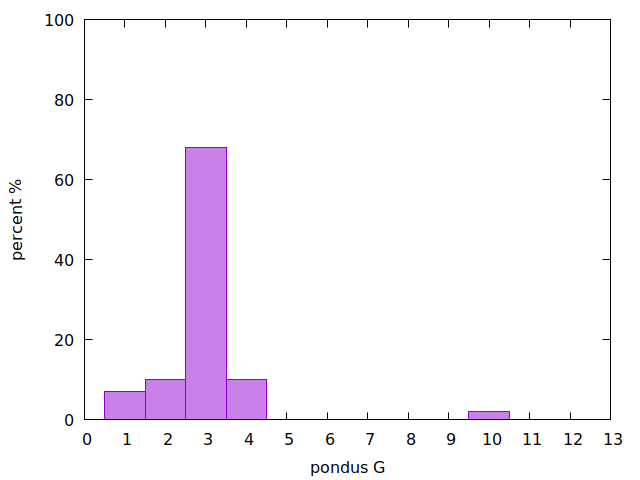
\includegraphics[width=\textwidth]{Pics/iv/iv-199-acoh.png}
        \caption{iv acoh} \label{fig:iv-acoh}
    \end{subfigure}
    \begin{subfigure}{.3\textwidth}
        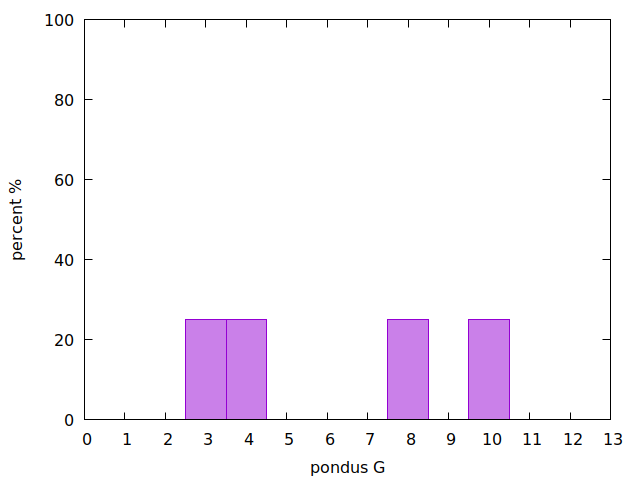
\includegraphics[width=\textwidth]{Pics/iv/iv-201-acoh-ipo.png}
        \caption{iv acoh ipo} \label{fig:iv-acoh-ipo}
    \end{subfigure}
    \begin{subfigure}{.3\textwidth}
        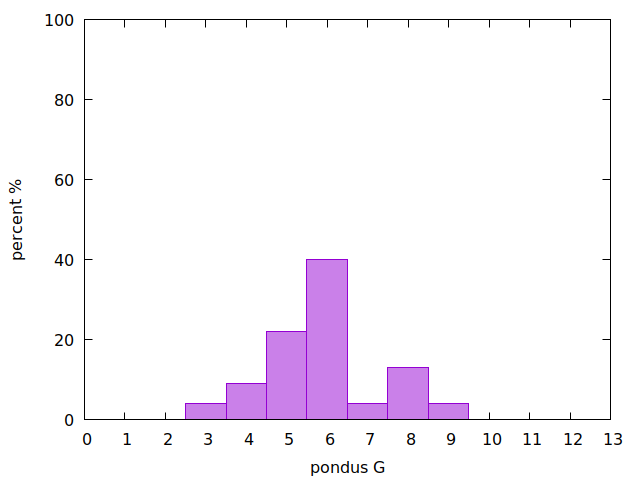
\includegraphics[width=\textwidth]{Pics/iv/iv-192-ipo.png}
        \caption{ipo} \label{fig:ipo}
    \end{subfigure}
    \caption{iv of 6x4F} \label{fig:iv-ipo}
\end{figure}

%\iffalse
%%%%%%%%%%%%%%%%%%%%%%%%%%%%%%%%%%%%%%%%%%%%%%%%%%%%%%%%%%%
%%%%%%%%%%%%%%%%%%%%%%%%%%%%%%%%%%%%%%%%%%%%%%%%%%%%%%%%%%%
\subsubsection{Infra Red}

\begin{figure}
    \centering
    \begin{subfigure}{.49\textwidth}
        \centering
        \includegraphics[width=.99\textwidth]{Pics/ir-gt.png}
        \caption{Transmittance of \gls{zro} on glass} \label{fig:ir-gt}
    \end{subfigure}
    \begin{subfigure}{.49\textwidth}
        \centering
        \includegraphics[width=.99\textwidth]{Pics/ir-gr.png}
        \caption{reflectance of \gls{zro} on glass} \label{fig:ir-gr}
    \end{subfigure}
    \caption{IR} \label{fig:ir}
\end{figure}

In figure \ref{fig:ir-gt} transmission spectra of visible and \gls{nir} light can be seen. 
Each sample had different numbers of layers. 
The incident angle was 0 degree for each sample.
differnt numbers of layers of \gls{zro} on a glass slide with 0 degree incident angle. 
The more layers the more of the light is absorbed (800nm) by the \gls{zro} layers. 
%The trend is not monotonic due to inhomogenities in the sample???b
The thicker the layer is the more wavy the graph, which can be most likely be attributed to interferrence. 
This trend can also be observed in figure \ref{fig:ir-gr}
Figure \ref{fig:ir-gr} shows reflectance spectra of visible and \gls{nir} at an angle of 45 degrees. 
%\fi


%%%%%%%%%%%%%%%%%%%%%%%%%%%%%%%%%%%%%%%%%%%%%%%%%%%%%%%%%%%
%%%%%%%%%%%%%%%%%%%%%%%%%%%%%%%%%%%%%%%%%%%%%%%%%%%%%%%%%%%
\subsubsection{SEM}
\begin{figure}
    \centering
    \begin{subfigure}{.45\textwidth}
        \centering
        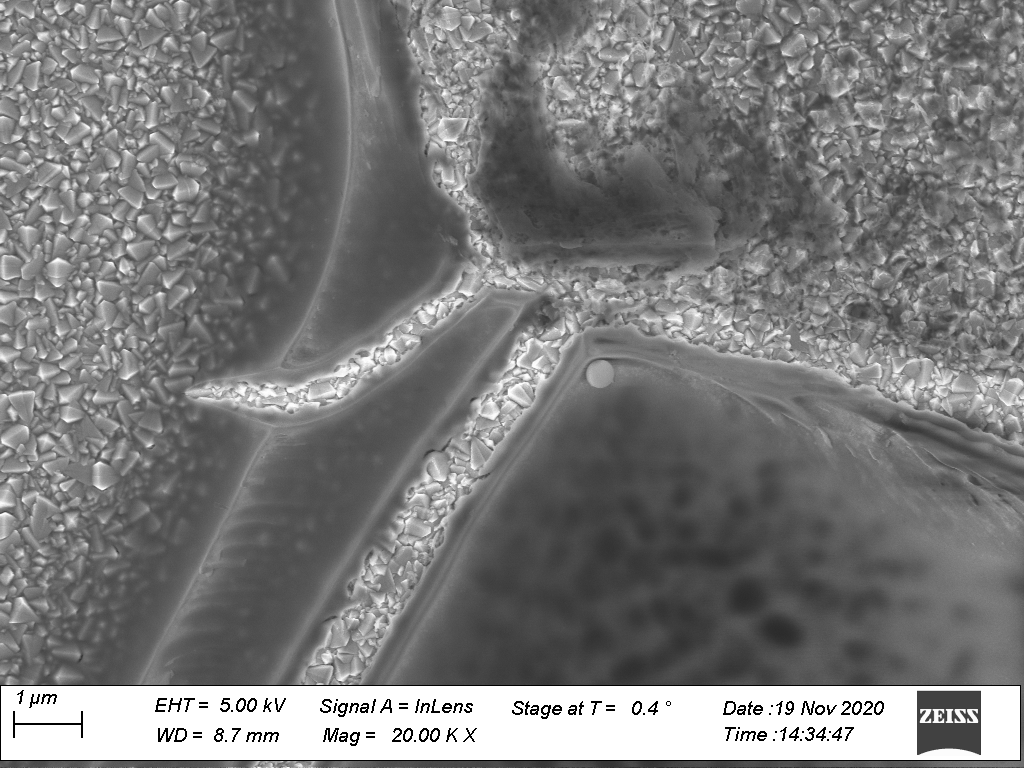
\includegraphics[width=.8\textwidth]{Pics/sem/071_fto_old_1x.png}
        \caption{71 fto old 1x} \label{fig:sem-old1}
    \end{subfigure}
    \begin{subfigure}{.45\textwidth}
        \centering
        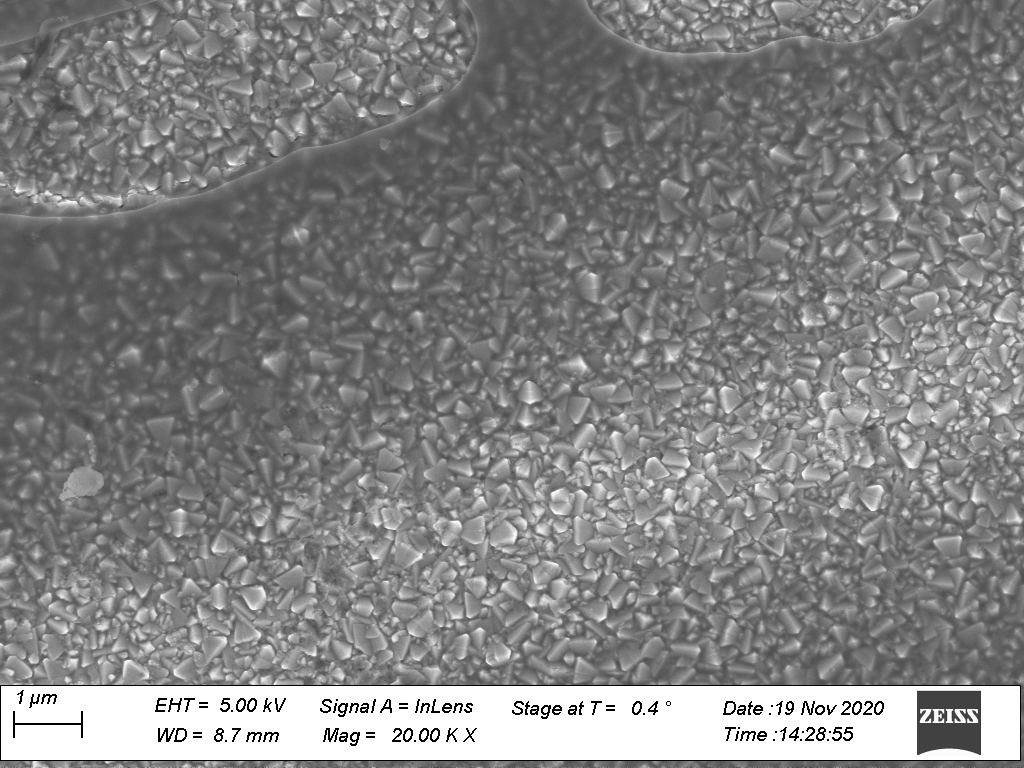
\includegraphics[width=.8\textwidth]{Pics/sem/071_fto_old_2x.png}
        \caption{71 fto old 2x} \label{fig:sem-old2}
    \end{subfigure}
    \begin{subfigure}{.45\textwidth}
        \centering
        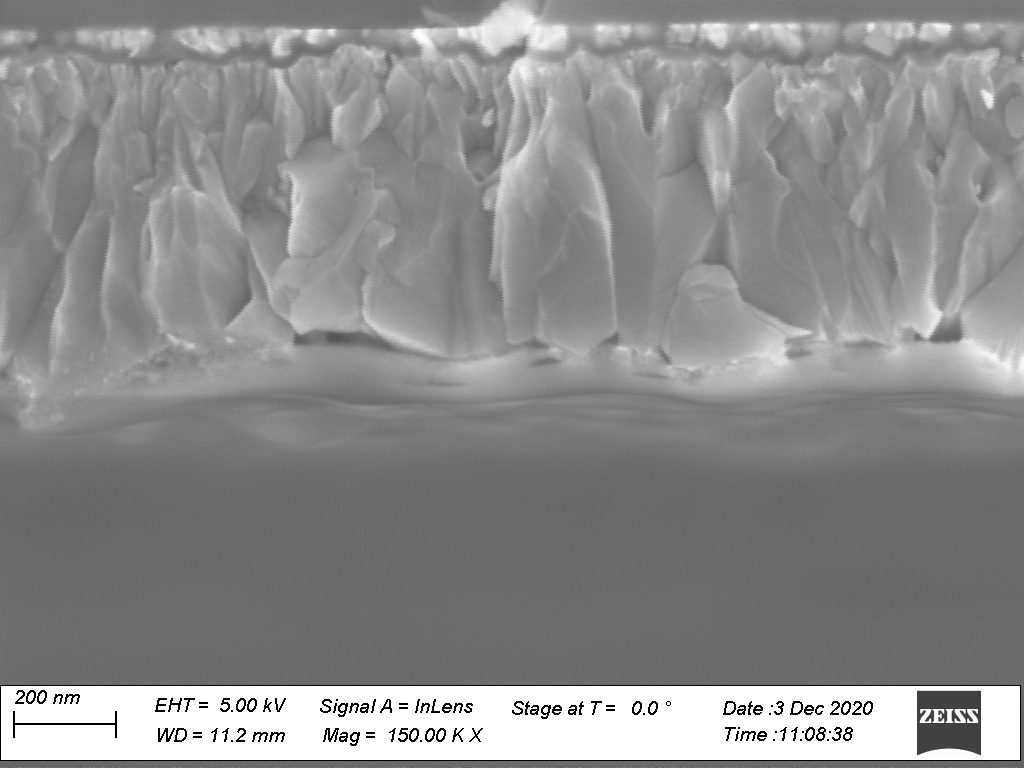
\includegraphics[width=.8\textwidth]{Pics/sem/115_fto_cs_1x.png}
        \caption{115 fto cs 1x} \label{fig:sem-cs1}
    \end{subfigure}
    \begin{subfigure}{.45\textwidth}
        \centering
        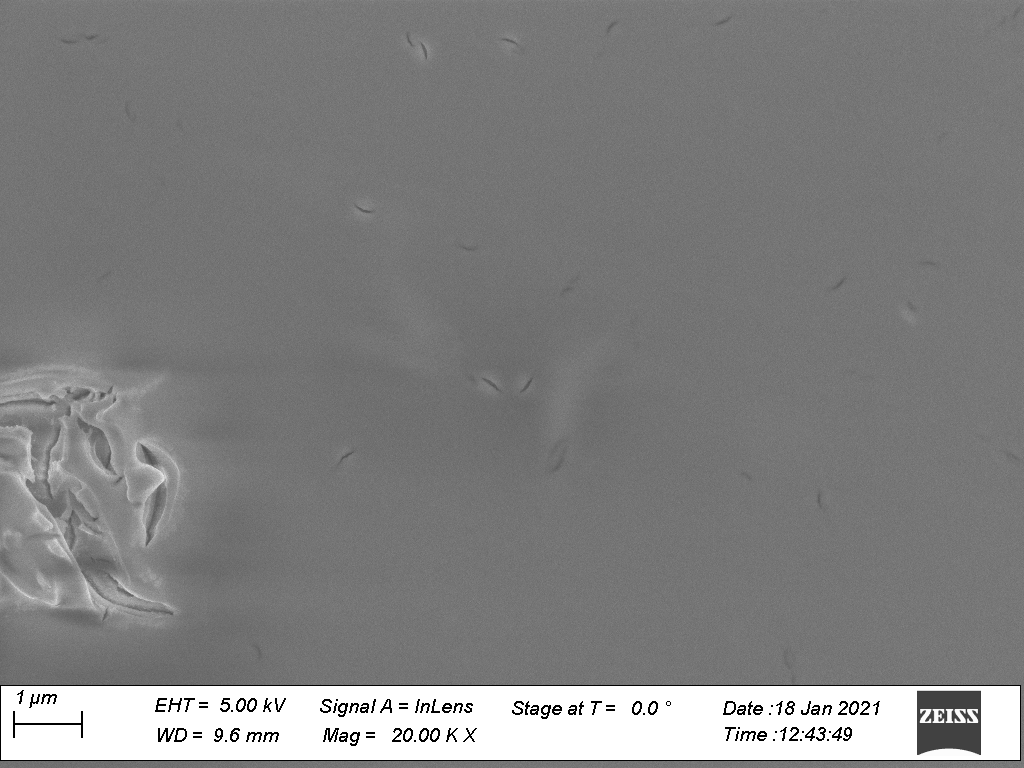
\includegraphics[width=.8\textwidth]{Pics/sem/147_steel_ph_10x.png}
        \caption{147 steel ph? 10x} \label{fig:sem-ph}
    \end{subfigure}
    \caption{sem}
    \label{fig:sem}
\end{figure}

The \gls{sem} pictures were not easy to take since we were trying to create an insulator 
and the quality of the picture relies on the conductance of the material's surface. 
This means that the better the quality of the resulting layer the more tedious it was to get/take a decent SEM image. 
Figures \ref{fig:sem-old1} and \ref{fig:sem-old2} shows ausschnitte of \gls{zro} (dark) on top of \gls{fto} (finely polycrystalline). 
These were the results of a single (figure \ref{fig:sem-old1}) and double (figure \ref{fig:sem-old2}) "layer" of the aquatic recipe. 
Large cracks and inhomogenity were part of (ausmachen) all samples created with the Anwar recipe; 
also/even after several/multiple/various alteration to the recipe. 

Figure \ref{fig:sem-cs1} shows the cross section of a single layers of \gls{zro} on \gls{fto} glass. 
The large crystalline \td{range} which makes up most of the topper/top part of the image is \gls{fto}. 
The úbergang to glass is gerade noch so zu sehen. 
On the lower kante of the \gls{fto} a circa 100nm thick homogeneous layer can be observed, \gls{zro} produced by buthanolic recipe inspired by Hu et al..

Figure \ref{fig:sem-ph} shows a top view of 10 layers of the buthanolic layer on top of a steel substrate. 
The large unregularity on the bottom left could darstellen a pin hole a (tiny) hole that reaches the substrate. 
These unregularites are rather the ausnahme. 
Alternatively, the small, hardly visible  irregularities verstreut across surface could darstellen such pin holes. 
These - I think - eher only are one layer deep irregularities since they are so haeufig 
and very little pin holes were observed on similar samples. 




%%%%%%%%%%%%%%%%%%%%%%%%%%%%%%%%%%%%%%%%%%%%%%%%%%%%%%%%%%%
%%%%%%%%%%%%%%%%%%%%%%%%%%%%%%%%%%%%%%%%%%%%%%%%%%%%%%%%%%%
\subsubsection{Current Voltage Curves} 
\begin{figure}
    \centering
    \begin{subfigure}{.3\textwidth}
        \includegraphics[width=\textwidth]{Pics/iv/log-154-good-3x4F.png}
        \caption{log good 3x4F} \label{fig:iv-log-good}
    \end{subfigure}
    \begin{subfigure}{.3\textwidth}
        \includegraphics[width=\textwidth]{Pics/iv/log-146-okay-10x1F.png}
        \caption{log okay 10x1F} \label{fig:iv-log-okay}
    \end{subfigure}
    \begin{subfigure}{.3\textwidth}
        \includegraphics[width=\textwidth]{Pics/iv/log-156-bad-3x3F.png}
        \caption{log bad 3x3F} \label{fig:iv-log-bad}
    \end{subfigure}
    \begin{subfigure}{.3\textwidth}
        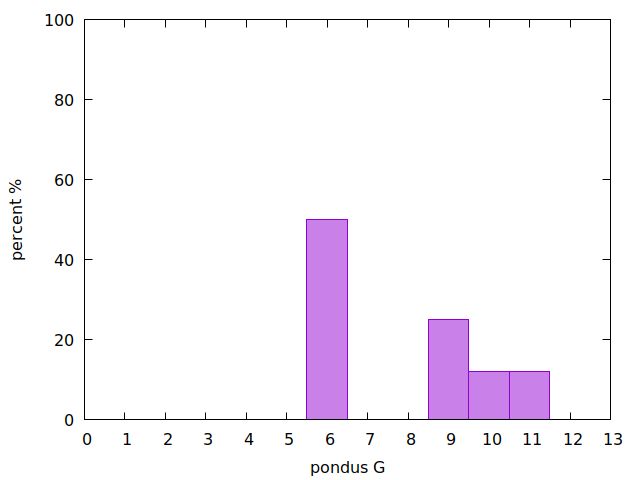
\includegraphics[width=\textwidth]{Pics/iv/stat-154-okay-3x4F.png}
        \caption{stat good 3x4F} \label{fig:iv-stat-good}
    \end{subfigure}
    \begin{subfigure}{.3\textwidth}
        \includegraphics[width=\textwidth]{Pics/iv/stat-146-good-10x1F.png}
        \caption{stat okay 10x1F} \label{fig:iv-stat-okay}
    \end{subfigure}
    \begin{subfigure}{.3\textwidth}
        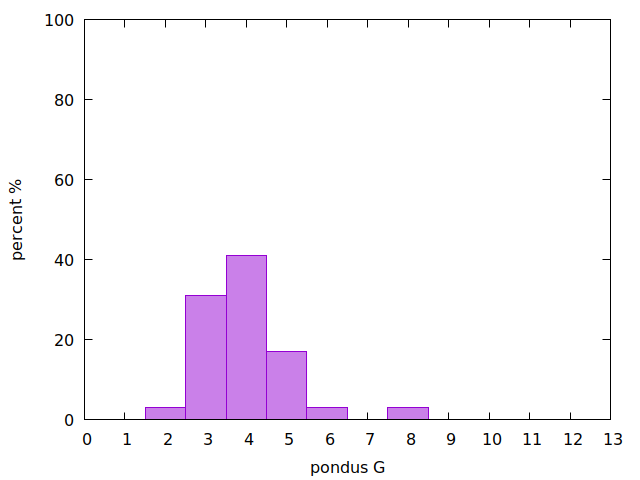
\includegraphics[width=\textwidth]{Pics/iv/stat-156-bad-3x3F.png}
        \caption{stat bad 3x3F} \label{fig:iv-stat-bad}
    \end{subfigure}
    \caption{maybe remove 146 and make 154 good AND set yrange [E-1:E-14] and show phd threshold} \label{fig:iv}
\end{figure}

%Figures \ref{fig:iv-log-good} and \ref{fig:iv-stat-good} are measurements from a good sample. 
Figure \ref{fig:iv-log-good} shows \gls{iv} curves in logarithmic scale of a good sample. 
Each line represents a I-V measurement at a distinct contact 
The highest voltages are around 
All of the curves show a max voltage of under \num{e-6} \SI{}{\volt}. 
And quite a few show hardly any current which is the ideal. 
For each measurement the conductivity (i.e. the gradient at V=0) was calculated (see section \ref{sec:eval}). 
Figure \ref{fig:iv-stat-good} shows the distribution of gradients. 

Figures \ref{fig:iv-log-okay} and \ref{fig:iv-stat-okay} show measurements from moderate sample. 
Most of the \gls{iv}s have a maximum voltage of under \num{e-6} V, but there are some so called pin holes. 

Finally, figures \ref{fig:iv-log-bad} and \ref{fig:iv-stat-bad} show a sample where all 
measurement exhibit relatively high voltages. Which indicates a bad overall \gls{zro} layer. 

%%%%%%%%%%%%%%%%%%%%%%%%%%%%%%%%%%%%%%%%%%%%%%%%%%%%%%%%%%%
%%%%%%%%%%%%%%%%%%%%%%%%%%%%%%%%%%%%%%%%%%%%%%%%%%%%%%%%%%%
\subsubsection{XRD}
\begin{figure}
	\centering
	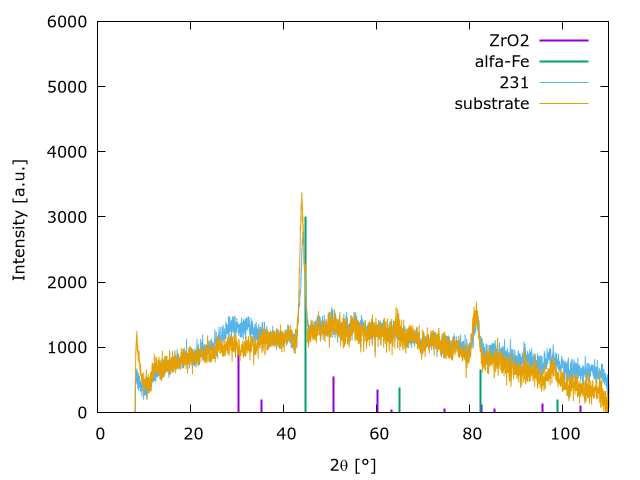
\includegraphics[width=\picwidth]{Pics/xrd.png}
	\caption{XRD spectra}
	\label{fig:xrd}
\end{figure}

In figure \ref{fig:xrd} the two strongest $\alpha$-Fe peaks can be seen clearly. 
The highest peak of \gls{zro} is very \td{broadened} and is therefore not as distinct. 
This wideness is is due to polycristalinity/amorphness of the material which is \td{erwartet due} to the sol-gel creation process. 

%%%%%%%%%%%%%%%%%%%%%%%%%%%%%%%%%%%%%%%%%%%%%%%%%%%%%%%%%%%
%%%%%%%%%%%%%%%%%%%%%%%%%%%%%%%%%%%%%%%%%%%%%%%%%%%%%%%%%%%
\subsubsection{Preoptimization}
The doctor blading velocity (i.e. the velocity with which the blade moves and spreads the sol over the sample) 
was varied during preoptimization. 
The slower the \gls{db} velocity the more \td{homogeneously} the solution evaporated. 
If the \gls{db} was \td{too slow (lt 1 mm/s)} the surface tension pulled solvent over the sample without \td{leaving was zurk/forming a gel.}
\td{deposition because miniscus is pulling liquid off the substrate.}
Additionally the temperature while doctor blading affects the resulting layer together with the \gls{db} velocity. 

\td{Assumption: Ideally solution evaporate shortly after DB but not before}
due to the boiling point of \gls{buoh} at 117 C\cite{ncbi1butanol} the room temperature to 80 C were used as temperature during \gls{db}.
- p76, 146 (10x1F) good, 154 (3x4F) okay, 156 (3x3F) bad visualisation

